\documentclass[parskip=full,11pt]{scrartcl}

\usepackage[utf8]{inputenc}

%\title{Simulator für wiederholte Spiele}
%\author{Sebastian Feurer, Peter Koepernik, Luc Mercatoris,\\Christian Schorr, Pierre Toussing}

% section numbers in margins:
\renewcommand\sectionlinesformat[4]{\makebox[0pt][r]{#3}#4}

% header & footer
\usepackage{scrlayer-scrpage}
\lofoot{\today}
\refoot{\today}
\pagestyle{scrheadings}

\usepackage[sfdefault,light]{roboto}
\usepackage[T1]{fontenc}
%\usepackage[german]{babel}
\usepackage[english]{babel}
\usepackage[yyyymmdd]{datetime} % must be after babel
\renewcommand{\dateseparator}{-} % ISO8601 date format
\usepackage{hyperref}
\usepackage{bbm}
\usepackage{amsmath} % for $\text{}$
\usepackage{amssymb}
\usepackage[nameinlink]{cleveref}
\crefname{figure}{Abb}{Abb}
\usepackage[section]{placeins}
\usepackage{xcolor}
\usepackage{graphicx}
\usepackage{subfig}
\usepackage{float} % für Fließumgebungen; Platzierung H verschiebt nicht
\usepackage{multirow}
\restylefloat{figure}
\hypersetup{
	pdftitle={Entwurf},
	bookmarks=true,
}
\usepackage{csquotes}

\newcommand\urlpart[2]{$\underbrace{\text{\texttt{#1}}}_{\text{#2}}$}

\usepackage{pflichtenheft}

\usepackage[nonumberlist]{glossaries}

\usepackage[T1]{fontenc}
\usepackage[scaled=0.85]{beramono}

\begin{document}
\begin{titlepage}
	\centering
	\vspace*{5cm}
	
\includegraphics[width = 0.7\linewidth]{images/Logos/loop.png}\par
	{\huge\bfseries Ein Simulator für wiederholte Spiele\par}
	%\vspace{1cm}
	{\Large Entwurfsdokument\par}
	\vspace{2cm}
	{\Large\itshape Sebastian Feurer, Peter Koepernik, Luc Mercatoris,\\Christian Schorr, Pierre Toussing\par}
	\vfill
	{\large \today\par}
\end{titlepage}

%\tableofcontents
%\pagebreak

\section{Introduction}
This document contains the design for \enquote{loop}, a simulation software for repeated games, as described in the \textit{Pflichtenheft}.

The object-oriented architecture of the project follows the model-view-controller (MVC) pattern, thus consists of three main packages: \texttt{view}, \texttt{controller} and \texttt{model}. The communication between view and model relies solely on the controller, hence the entirety of the model is decoupled from the view.

\begin{figure}[h]
	\centering
	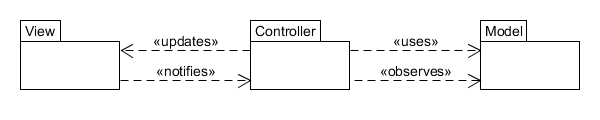
\includegraphics[width=0.7\linewidth]{images/package_diagram_overview.png}
	\caption{Sketch of the package structure. The view notifies the controller when the user interacts with the UI, who then uses the model to carry out tasks requested by the user. The controller observes the model to notice changes in the models computations and updates the view accordingly.}
	\label{package_overview}
\end{figure}

\subsection{The view}
Since the user interface (UI) of the program was designed using the UI-Builder \textit{NAMEEINFÜGEN}, the \texttt{view}-package contains mainly auto-generated classes provided by \textit{NAMEEINFÜGEN}.

The communication between view and model relies solely on the controller. Each window in the view has one controller assigned to it, that will be instantiated automatically when the window is opened and handles any input performed by the user.

\subsection{The controller}
The controller consists of a tree-like class hierarchy. At the top resides the \texttt{HeadController}, who is associated with the main window and thus instantiated when the program starts. The other controllers are arranged below and associated with the different popup windows such as the configuration- or the strategy creation window.

When the user requests a task that requires the involvement of the model (such as starting a simulation or saving a configuration file), the \texttt{HeadController} invokes the model, observes it for updates in its computation progress and updates the view accordingly.

When the user navigates to other windows the \texttt{HeadController} opens them and observes the corresponding controller so it can relay tasks to the model or close the window if needed.

\subsection{The model}
The model contains the \texttt{Simulator} class, which provides means for starting and stopping simulations to given configurations.

Since the execution of a simulation might take a considerable amount of time, depending on the configuration and the accessible hardware resources, simulations will be started asynchronously and an instance of the \texttt{SimulationResult} class will be returned instantly, which will be filled with the results of the single iterations as they finish. The \texttt{SimulationResult} offers a possibility to observe it in the sense that a method may be registered as functional interface which will be called whenever an iteration finishes.

The execution of a single iteration itself is encapsulated in the \texttt{SimulationEngine} class. It receives an instance of the \texttt{Configuation} class and returns the result of the simulation as an instance of the \texttt{IterationResult}. The simulation process is implemented as a template method and the configuration is queried whenever a varaible event such as the strategy adjustion or the agent pairing occurs.

The model contains interfaces representing those variable events and provides implementations for the mechanisms and algorithms described in the \textit{Pflichtenheft}. The user may implement those interfaces himself and integrate them in the program using the plug-in system which is also part of the model.

\section{Spezifikationsänderungen}

\subsection{Populationen}
Das Konzept von Gruppen und Segmenten wurde überarbeitet. Die Gesamtheit der Gruppen, Segmente, sowie deren Größen und Einstellungen (bis auf Multikonfiguration) heißt nun eine \enquote{Population}. Die Konfiguration von Gruppen und Populationen wurde aus dem Konfigurationsfenster ausgelagert. Wie zur Strategie- und Stufenspielerstellung gibt es nun Fenster zur Erstellung einzelner Gruppen und Populationen.

\textbf{Gruppenerstellung:}
Im Gruppenerstellungsfenster können ein Name und eine Beschreibung der Gruppe eingetragen werden. Weiter können Anzahl und Größe von Segmenten sowie jeweils Strategie- und Kapitalverteilung eingestellt werden. Weiterhin kann eine Gruppe per Checkbox als \enquote{kohärent} deklariert werden (siehe \cref{?}). Diese Checkbox ist voreingestellt aktiviert. Wird sie deaktiviert, so identifizieren sich Agenten dieser Gruppe gegenseitig nicht mehr als Agenten derselben Gruppe. Diese Funktionalität realisiert das Konzept der \enquote{gruppenlosen Agenten}. Eine fertig konfigurierte Gruppe kann als Datei exportiert und eine als Datei exportierte Gruppe kann importiert werden.

\textbf{Populationserstellung:}
Im Populationserstellungsfenster können ein Name sowie eine Beschreibung der Population eingetragen werden. Dann können \(1\) bis \(16\) der selbst erstellten oder von vornherein im Programm hinterlegten Gruppen hinzugefügt werden. Für jede Gruppe können die Anzahl der Mitglieder über ein Textfeld eingegeben werden (siehe \cref{?}). Eine fertig konfigurierte Population kann als Datei exportiert und eine als Datei exportierte Population kann importiert werden.

Das Konfigurationsfenster ist nun nicht mehr in drei Bereiche unterteilt. Statt der Gruppeneinstellungen befindet sich nun zwischen den nun verschmolzenen, ehemaligen \enquote{Grund-} und \enquote{Erweiterten Einstellungen} nur noch ein Dropdown-Menü mit der Betitelung \enquote{Population} (siehe \cref{?}). Hier kann eine der selbst erstellten oder von vornherein im Programm hinterlegten Populationen ausgewählt werden. Unter dem Dropdown-Menü kann ein Abschnitt ausgeklappt werden, der die Zusammensetzung der Population zeigt (siehe \cref{?}). Dieser hat dieselbe Form wie die ehemaligen Gruppeneinstellungen, mit dem Unterschied, dass keine Modifikationen mehr vorgenommen werden können. Per Checkbox kann dort die \enquote{Multikonfiguration} für Segmente und Gruppen wie zuvor aktiviert werden.

\subsection{Strategien}
Die Liste aller Variablen, die in einer Strategie als Literal vorkommen können wurde um die folgenden erweitert:

\begin{itemize}
\item B hat bei bisherigen Spielen zwischen B und Agenten derselben Gruppenzugehörigkeit wie A (im aktuellen Adaptionsschritt) immer/nie/letztes Mal/wenigstens einmal kooperiert
\item B hat bei bisherigen Spielen zwischen B und Agenten mit ähnlichem aktuellen Kapital wie A (im aktuellen Adaptionsschritt) immer/nie/letztes Mal/wenigstens einmal kooperiert
\end{itemize}

\subsection{Plugin system}

A plugin system which allows to dynamicly load new functionality at runtime has been added. This gives the user the flexibility to implement new algorithms and mechanism that can be used in simulations. The following parameter set can be extended via plugins:
\begin{itemize} \itemsep -10pt
	\item the equilibrium criterion mechanism
	\item the success quantifier mechanism
	\item the strategy adjuster mechanism
	\item the pair builder algorithm
	\item the discrete distribution algorithm
\end{itemize}

Furthermore it is possible to make the plugins user configurable from the configuration window. Therefor plugins can provide a renderer which creates a user control that gets embedded into the configuration window.\\
Plugins are loaded automatically at the program start.

\section{Pakete und Klassen}

\subsection{Paket \texttt{edu.kit.loop}}

\subsubsection{Class \texttt{Main extends javafx.application.Application}}

This class contains the main method (entry point) of the program and initializes the main-window.

Methoden:
\begin{itemize}\itemsep -10pt
\item \underline{\texttt{void main(String[] args))}}
\item[] The entry point of the application. Loads the UI and starts the window.
\item[] \texttt{args}: the commandline arguments. (unused)
\end{itemize}

\subsection{Paket \texttt{edu.kit.loop.model}}
Das Modell beinhaltet Klassen und Methoden zum Starten und Abbrechen von Simulationen, sowie zum Erstellen und Speichern von Konfigurationen, Stufenspielen, Strategien und Populationen.

\subsubsection{Class \texttt{UserConfiguration}}
Implements: \texttt{java.io.Serializable}

Diese Klasse repräsentiert eine vom Nutzer erstellte Konfiguration. Sie bietet Methoden zum Lesen aller zugehörigen Parameter.

Konstruktoren:
\begin{itemize}\itemsep -10pt
\item \texttt{UserConfiguration(String gameName, int agentCount, int roundCount, int iterationCount, List<String> availableStrategyNames, boolean mixedAllowed, String populationName, String pairBuilderName, List<double> pairBuilderParameters, String successQuantifierName, List<double> successQuantifierName, String strategyAdjusterName, List<double> strategyAdjusterParameters, String\\ equilibriumCriterionName, List<double> equilibriumCriterionParameters, int maxAdapts, boolean isMulticonfiguration, String variableParameterName, double startValue, double endValue, double stepSize)}
\item[] Creates a new \texttt{UserConfiguration} with the given parameters
\item[] \texttt{gameName}: the name of the game
\item[] \texttt{agentCount}: the amount of agents
\item[] \texttt{roundCount}: the amount of rounds per adaptionstep
\item[] \texttt{iterationCount}: the amount of iterations
\item[] \texttt{availableStrategyNames}: a list with the names of all allowed strategies
\item[] \texttt{mixedAllowed}: \texttt{true}, if mixed strategies are allowed, \texttt{false} otherwise.
\item[] \texttt{populationName}: the name of the population
\item[] \texttt{pairBuilderNames}: the name of the pair builder
\item[] \texttt{pairBuilderParameters}: a list with the values of the parameters of the pair builder
\item[] \texttt{successQuantifierNames}: the name of the success quantifier
\item[] \texttt{successQuantifierParameters}: a list with the values of the parameters of the success quantifier
\item[] \texttt{strategyAdjusterName}: the name of the strategy adjuster
\item[] \texttt{strategyAdjusterParameters}: a list with the values of the parameters of the strategy adjuster
\item[] \texttt{equilibriumCriterionName}: the name of the equilibrium criterion
\item[] \texttt{equilibriumCriterionParameters}: a list with the values of the parameters of the equilibrium criterion
\item[] \texttt{maxAdapts}: the maximum amount of simulated adaption steps per iteration
\item[] \texttt{isMulticonfiguration}: \texttt{true}, if this is a multiconfiguration, \texttt{false} otherwise
\item[] \texttt{variableParameterName}: the name of the multiconfiguration parameter, if this is a multiconfiguration, \texttt{""} otherwise
\item[] \texttt{startValue}: the starting value of the multiconfiguration parameter, if this is a multiconfiguration, \(0\) otherwise
\item[] \texttt{endValue}: the end value of the multiconfiguration parameter, if this is a multiconfiguration, \(0\) otherwise
\item[] \texttt{stepSize}: the step size of the multiconfiguration parameter, if this is a multiconfiguration, \(0\) otherwise
\end{itemize}

Methoden:
\begin{itemize}\itemsep -10pt
	\item \texttt{String getGameName()}
	\item[] Returns the name of the game of this configuration
	\item[] Returns: the name of the game of this configuration
	
	\item \texttt{int getAgentCount()}
	\item[] Returns the amount of agents in this configuration
	\item[] Returns: the amount of agents in this configuration
	
	\item \texttt{int getRoundCount()}
	\item[] Returns the amount of rounds per adaption step in this configuration
	\item[] Returns: the amount of rounds per adaption step in this configuration
	
	\item \texttt{int getIterationCount()}
	\item[] Returns the amount of iterations in this configuration
	\item[] Returns: the amount of iterations in this configuration
	
	\item \texttt{List<String> getAvailableStrategyNames()}
	\item[] Returns a list with names of all available strategies in this configuration
	\item[] Returns: a list with names of all available strategies in this configuration
	
	\item \texttt{boolean getMixedAllowed()}
	\item[] Returns, whether mixed strategies are allowed in this configuration
	\item[] Returns: \texttt{true}, if mixed strategies are allowed in this configuration; \texttt{false} otherwise
	
	\item \texttt{String getPopulationName()}
	\item[] Returns the name of the \texttt{Population} of this configuration
	\item[] Returns: a list with the names of all populations in this configuration
	
	\item \texttt{String getPairBuilderName()}
	\item[] Returns the name of the \texttt{PairBuilder} of this configuration
	\item[] Returns: the name of the \texttt{PairBuilder} of this configuration
	
	\item \texttt{List<double> getPairBuilderParameters()}
	\item[] Returns a list with the values of the parameters of the \texttt{PairBuilder} of this configuration
	\item[] Returns: a list with the values of the parameters of the \texttt{PairBuilder} of this configuration
	
	\item \texttt{String getSuccessQuantifierName()}
	\item[] Returns the name of the \texttt{SuccessQuantifier} of this configuration
	\item[] Returns: the name of the \texttt{SuccessQuantifier} of this configuration
	
	\item \texttt{List<double> getSuccessQuantifierParameters()}
	\item[] Returns a list with the values of the parameters of the \texttt{SuccessQuantifier} of this configuration
	\item[] Returns: a list with the values of the parameters of the \texttt{SuccessQuantifier} of this configuration
	
	\item \texttt{String getStrategyAdjusterName()}
	\item[] Returns the name of the \texttt{PairBuilder} of this configuration.
	\item[] Returns: the name of the \texttt{PairBuilder} of this configuration
	
	\item \texttt{List<double> getStrategyAdjusterParameters()}
	\item[] Returns a list with the values of the parameters of the \texttt{StrategyAdjuster} of this configuration
	\item[] Returns: a list with the values of the parameters of the \texttt{StrategyAdjuster} of this configuration
	
	
	\item \texttt{String getEquilibriumCriterionName()}
	\item[] Returns the name of the \texttt{EquilibriumCriterion} of this configuration.
	\item[] Returns: the name of the \texttt{EquilibriumCriterion} of this configuration.
	
	\item \texttt{List<double> getEquilibriumParameters()}
	\item[] Returns a list with the values of the parameters of the \texttt{EquilibriumCriterion} of this configuration
	\item[] Returns: a list with the values of the parameters of the \texttt{EquilibriumCriterion} of this configuration
	
	\item \texttt{int getMaxAdapts()}
	\item[] Returns the maximum amount of simulated adaption steps per iteration in this configuration
	\item[] Returns: the maximum amount of simulated adaption steps per iteration in this configuration
	
	\item \texttt{boolean isMulticonfiguration()}
	\item[] Returns whether this is a multiconfiguration.
	\item[] Returns: \texttt{true}, if this is a multiconfiguration, \texttt{false} otherwise
	
	\item \texttt{String getVariableParameterName()}
	\item[] Returns the name of the multiconfiguration parameter of this configuration, if this is a multiconfiguration; \texttt{""} otherwise.
	\item[] Returns: the name of the multiconfiguration parameter of this configuration, if this is a multiconfiguration; \texttt{""} otherwise
	
	\item \texttt{double getStartValue()}
	\item[] Returns the starting value of the multiconfiguration parameter of this configuration, if this is a multiconfiguration; \(0\) otherwise.
	\item[] Returns: the starting value of the multiconfiguration parameter of this configuration, if this is a multiconfiguration; \(0\) otherwise
	
	\item \texttt{double getEndValue()}
	\item[] Returns the end value of the multiconfiguration parameter of this configuration, if this is a multiconfiguration; \(0\) otherwise.
	\item[] Returns: the end value of the multiconfiguration parameter of this configuration, if this is a multiconfiguration; \(0\) otherwise
	
	\item \texttt{double getStepSize()}
	\item[] Returns the step size of the multiconfiguration parameter of this configuration, if this is a multiconfiguration; \(0\) otherwise.
	\item[] Returns: the step size of the multiconfiguration parameter of this configuration, if this is a multiconfiguration; \(0\) otherwise
	
	
\end{itemize}


\subsubsection{Class \texttt{Configuration}}
Diese Klasse repräsentiert die elementare Konfiguration einer einzelnen Wiederholung und enthält alle Informationen zum Start einer solchen:
\begin{itemize}\itemsep -10pt
\item Stufenspiel
\item Anzahl von Agenten
\item Runden pro Adaptionsschritt
\item Ob gemischte Strategien zugelassen sind
\item Gruppen-/Segmenteinteilungen
\item Kapital- und Strategieinitialisierung der Segmente
\item Agentenpaarung
\item Erfolgsquantifizierung
\item Adaptionsmechanismus
\item Gleichgewichtskriterium
\item Maximale Zahl von Adaptionsschritten
\end{itemize}

Konstruktoren:
\begin{itemize}\itemsep -10pt
\item \texttt{Configuration(Game game, int roundCount, boolean mixedStrategies, Collection<Segment> segments, PairBuilder pairBuilder, SuccessQuantifier successQuantifier, SrategyAdjuster strategyAdjuster, EquilibriumCriterion equilibriumCriterion, int maxAdapts)}
\item[] Creates a new \texttt{Configuration} with the given parameters.
\item[] \texttt{game}: the game of this configuration
\item[] \texttt{roundCount}: the amount of rounds per adaption step in this configuration
\item[] \texttt{mixedStrategies}: \texttt{true}, if mixed strategies are allowed in this configuration, \texttt{false} otherwise
\item[] \texttt{segments}: all segments of this configuration
\item[] \texttt{pairBuilder}: the \texttt{PairBuilder} of this configuration
\item[] \texttt{successQuantifier}: the \texttt{SuccessQuantifier} of this configuration
\item[] \texttt{strategyAdjuster}: the \texttt{StrategyAdjuster} of this configuration
\item[] \texttt{equilibriumCriterion}: the \texttt{EquilibriumCriterion} of this configuration
\item[] \texttt{maxAdapts}: the maximum amount of simulated adaption steps per iteration in this configuration
\end{itemize}

Methoden:
\begin{itemize}\itemsep -10pt
\item \texttt{Game getGame()}
\item[] Returns the game of this configuration
\item[] Returns: the game of this configuration

\item \texttt{int getAgentCount()}
\item[] Returns the amount of agents in this configuration
\item[] Returns: the amount of agents in this configuration

\item \texttt{int getRoundCount()}
\item[] Returns the amount of rounds per adaption step in this configuration
\item[] Returns: the amount of rounds per adaption step in this configuration

\item \texttt{boolean allowsMixedStrategies()}
\item[] Returns, whether mixed strategies are allowed in this configuration.
\item[] Returns: \texttt{true}, if mixed strategies are allowed in this configuration, \texttt{false} otherwise

\item \texttt{Collection<Segment> getSegments()}
\item[] Returns all segments belonging to this configuration
\item[] Returns: all segments belonging to this configuration as \texttt{Collection<Segment>}

\item \texttt{PairBuilder getPairBuilder()}
\item[] Returns the \texttt{pairBuilder} of this configuration.
\item[] Returns: the \texttt{pairBuilder} of this configuration

\item \texttt{SuccessQuantifier getSuccessQuantifier()}
\item[] Returns the \texttt{SuccessQuantifier} of this configuration.
\item[] Returns: the \texttt{SuccessQuantifier} of this configuration

\item \texttt{StrategyAdjuster getStrategyAdjuster()}
\item[] Returns the \texttt{StrategyAdjuster} of this configuration.
\item[] Returns: the \texttt{StrategyAdjuster} of this configuration

\item \texttt{EquilibriumCriterion getEquilibriumCriterion()}
\item[] Returns the \texttt{EquilibriumCriterion} of this configuration.
\item[] Returns: the \texttt{EquilibriumCriterion} of this configuration

\item \texttt{int getMaxAdapts()}
\item[] Returns the maximum amount of simulated adaption steps per iteration in this configuration
\item[] Returns: the maximum amount of simulated adaption steps per iteration in this configuration
\end{itemize}

\subsubsection{Interface \texttt{Nameable}}

Implementierungen dieses Interface haben einen Namen und eine Beschreibung, die in Form von \texttt{String}s abgefragt werden können.

Methoden:
\begin{itemize}\itemsep -10pt
\item \texttt{String getName()}
\item[] Returns the name of this object.
\item[] Returns: the name of this object

\item \texttt{String getDescription()}
\item[] Returns the description of this object.
\item[] Returns: the description of this object
\end{itemize}

\subsubsection{Class \texttt{Population}}
Implements: \texttt{Nameable}

Diese Klasse repräsentiert eine Population. Sie bietet Methoden zur Abfrage von Größe und Gruppenzusammensetzung.

Konstruktoren:
\begin{itemize}\itemsep -10pt
\item \texttt{Population(String name, String description, List<Group> groups, List<Integer> groupSizes)}
\item[] Creates a new \texttt{Population} with name, description and \texttt{Group} composition as given.
\item[] \texttt{name}: the name of this population
\item[] \texttt{description}: the description of this population
\item[] \texttt{groups}: the groups this population is composed of
\item[] \texttt{groupSizes}: the sizes of the groups, in the same order as the groups themselves
\end{itemize}

Methoden:
\begin{itemize}\itemsep -10pt
\item \texttt{int getSize()}
\item[] Returns the size of this population.
\item[] Returns: the size of this population

\item \texttt{List<Group> getGroups()}
\item[] Returns the groups this population is composed of.
\item[] Returns: the groups this population is composed of

\item \texttt{int getGroupSize(Group group)}
\item[] Returns the size of the given group if it is part of this population, \(0\) otherwise.
\item[] \texttt{group}: the group, whose size shall be returned
\item[] Returns: the size of the given group if it is part of this population, \(0\) otherwise

\item \texttt{int getGroupCount()}
\item[] Returns the amount of groups in this population
\item[] Returns: the amount of groups in this population
\end{itemize}

\subsubsection{Class \texttt{Group}}
Implements: \texttt{Nameable}

Diese Klasse repräsentiert eine Gruppe. Sie bietet Methoden zur Abfrage von Segmentzusammensetzung und Kohäsion.

Konstruktoren:
\begin{itemize}\itemsep -10pt
\item \texttt{Group(String name, String description, List<Segment> segments, List<Double> segmentSizes, boolean isCohesive)}
\item[] Creates a new \texttt{Group} with name, description and \texttt{Segment} composition as given
\item[] \texttt{name}: the name of this group
\item[] \texttt{description}: the description of this group
\item[] \texttt{segments}: the segments this group is composed of
\item[] \texttt{segmentSizes}: the relative sizes of the segments in the same order as the segments themselves
\item[] \texttt{isCohesive}: indicates whether this group is cohesive
\end{itemize}

Methoden:
\begin{itemize}\itemsep -10pt
\item \texttt{List<Segment> getSegments()}
\item[] Returns a list of the segments this group is composed of.
\item[] Returns: a list of the segments this group is composed of

\item \texttt{double getSegmentSize(Segment segment)}
\item[] Returns the relative size of the given \texttt{Segment} if it is part of this group, \(0\) otherwise.
\item[] \texttt{segment}: the segment whose relative size shall be returned
\item[] Returns: the relative size of the given \texttt{Segment} if it is part of this group, \(0\) otherwise

\item \texttt{int getSegmentCount()}
\item[] Returns the amount of segments in this group.
\item[] Returns: the amount of segments in this group

\item \texttt{boolean isCohesive()}
\item[] Returns whether this group is cohesive.
\item[] Returns: \texttt{true} if this group is cohesive, \texttt{false} otherwise
\end{itemize}

\subsubsection{Class \texttt{Segment}}

Diese Klasse repräsentiert ein Segment. Es bietet Methoden zur Abfrage von Kapital- und Strategieverteilung. Dabei werden lediglich die Namen der Kapitalverteilung sowie der verschiedenen Strategien gespeichert, die zu der entsprechenden \texttt{DiscreteDistribution} bzw. den entsprechenden \texttt{Strategy}s im zentralen Repository korrespondieren.

Konstruktoren:
\begin{itemize}\itemsep -10pt
\item \texttt{Segment(String capitalDistributionName, Collection<String> strategyNames)}
\item[] Creates a new \texttt{Segment} with the given capital- and strategy distribution
\item[] \texttt{capitalDistributionName}: the name of the capital distribution of this segment
\item[] \texttt{strategyNames}: the names of the strategies in the strategy distribution of this segment
\end{itemize}

Methoden:
\begin{itemize}\itemsep -10pt
\item \texttt{String getCapitalDistributionName()}
\item[] Returns the name of the capital distribution of this segment.
\item[] Returns: the name of the capital distribution of this segment

\item \texttt{Collection<String> getStrategyNames()}
\item[] Returns the names of the strategies in the strategy distribution of this segment.
\item[] Returns: the names of the strategies in the strategy distribution of this segment
\end{itemize}


\subsection{Paket \texttt{edu.kit.loop.model.simulator}}
Dieses Paket enthält das Interface \texttt{Simulator}. Dieses bietet eine Schnittstelle zum Starten und Abbrechen von Simulationen. Beim Start einer Simulation wird eine Referenz auf ein \texttt{Simulation}-Objekt zurückgegeben, über das der Ausführungsstatus und die Ergebnisse der Simulation abgefragt werden können.

\subsubsection{Class \texttt{SimulationResult}}
Ein \texttt{Simulation}-Objekt enthält Informationen zu einer gestarteten Simulation, etwa deren Konfiguration, Ausführungsstatus, \texttt{id} und gegebenenfalls die Ergebnisse der Simulation. Es wird von einem \texttt{Simulator} erzeugt und bereitgestellt, wenn eine Simulation gestartet wird.

Die Klasse unterscheidet nicht zwischen Multikonfigurationen und Nicht-Multikonfigurationen, geht also allgemein von mehreren zugrundeliegenden elementaren Konfigurationen aus.

Konstruktoren:
\begin{itemize} \itemsep -10pt
	\item \texttt{Simulation(UserConfiguration config, int id)}
	\item[] Creates a new \texttt{Simulation} with the given \texttt{UserConfiguration} and \texttt{id}.
	\item[] \texttt{config}: the configuration of this simulation
	\item[] \texttt{id}: the \texttt{id} of this simulation
\end{itemize}

Methoden:
\begin{itemize}\itemsep -10pt
	\item \texttt{protected void addIterationResult(IterationResult result, int i)}
	\item[] adds an \texttt{IterationResult} to the \texttt{i}-th elementary configuration of this simulation and triggers all registered actions
	\item[] \texttt{result}: the \texttt{IterationResult} that shall be added
	\item[] \texttt{i}: the elementary configuration to which the given \texttt{IterationResult} shall be added
	
	\item \texttt{protected void addSimulationEngineException()}
	\item[] adds an \texttt{SimulationEngineException} to this Simulaton and triggers all registered exception handler
	
	\item \texttt{void registerIterationFinished(BiConsumer<SimulationResutl,IterationResult> action)}
	\item[] Registers an action that will be executed every time an iteration of this simulation is finished. The \texttt{IterationResult} of the iteration as well as this instance will be passed as an argument to the action
	\item[] \texttt{action}: the action that shall be executed whenever an iteration finishes
	
	\item \texttt{void registerExceptionHandler(BiConsumer<SimulationResult,SimulationEngineException> handler)}
	\item[] Registers a handler that will be executed every time an exception corresponding to this simulation occurs
	\item[] \texttt{handler}: the handler that shall be executed whenever an exception occurs
	
	\item \texttt{List<IterationResult> getIterationResults(int i)}
	\item[] Returns a list of all yet available \texttt{IterationResult}s of iterations with the \texttt{i}-th elementary configuration.
	\item[] \texttt{i}: the elementary configuration, whose finished iterations shall be returned
	\item[] Returns: a list of all yet available \texttt{IterationResult}s of iterations with the \texttt{i}-th elementary configuration
	
	\item \texttt{UserConfiguration getUserConfiguration()}
	\item[] Returns the \texttt{UserConfiguration} of this simulation.
	\item[] Returns: the \texttt{UserConfiguration} of this simulation
	
	\item \texttt{int getConfigurationCount()}
	\item[] Returns the amount of elementary configurations of this simulation (\(1\) if this is not a multiconfiguration).
	\item[] Returns: the amount of elementary configurations of this simulation
	
	\item \texttt{int getId()}
	\item[] Returns the \texttt{id} of this simulation.
	\item[] Returns: the \texttt{id} of this simulation
\end{itemize}

\subsubsection{Interface \texttt{Simulator}}
Über einen Simulator können Simulationen gestartet und abgebrochen werden. Zum Starten einer Simulation muss dem \texttt{Simulator} eine \texttt{UserConfiguration} übergeben werden, die die durchzuführende Simulation spezifiziert. Daraufhin wird ein \texttt{Simulation}-Objekt erzeugt und zurückgegeben, über das der Ausführungsstatus und die Ergebnisse der gestarteten Simulation abgefragt werden können. Jeder Simulation wird beim Start eine eindeutige \texttt{id} zugewiesen.

Methoden:
\begin{itemize} \itemsep -10pt
	\item \texttt{SimulationResult startSimulation(UserConfiguration config)}
	\item[] Starts a new simulation with the given \texttt{UserConfiguration} and returns a handle to a \texttt{SimulationResult}-object for the started simulation.
	\item[]\texttt{config}: the configuration for which a simulation shall be started
	\item[] Returns: a handle to a \texttt{SimulationResult}-object for the started simulation
	\item[] Throws: \texttt{ConfigurationException} when the provided \texttt{UserConfiguration} is faulty
	
	\item \texttt{SimulationResult startSimulation(UserConfiguration config, Consumer<SimulationResult> action)}
	\item[] Starts a new simulation with the given \texttt{UserConfiguration} and returns a handle to a \texttt{SimulationResult}-object for the started simulation. Executes the given action with the \texttt{SimulationResult}-object passed as parameter when the started simulation is finished.
	\item[] \texttt{config}: the \texttt{UserConfiguration} a new simulation shall be started with
	\item[] \texttt{action}: the action that shall be executed when the simulation is finished
	\item[] Returns: a handle to a \texttt{SimulationResult}-object for the started simulation
	\item[] Throws: \texttt{ConfigurationException} when the provided \texttt{UserConfiguration} is faulty
	
	\item \texttt{boolean stopSimulation(SimulationResult sim)}
	\item[] Stop the execution of the given simulation if it is currently running.
	\item[] \texttt{sim}: the simulation whose execution shall be stopped
	\item[] Returns: \texttt{true}, if the execution of the simulation was successfully stopped, \texttt{false} otherwise
	
	\item \texttt{boolean stopSimulation(int id)}
	\item[] If a simulation with the given \texttt{id} is currently running, stop its execution.
	\item[] \texttt{id}: the \texttt{id} of the simulation that shall be stopped
	\item[] Returns: \texttt{true}, if the execution of the simulation was successfully stopped, \texttt{false} otherwise
	
	\item \texttt{void stopAllSimulation()}
	\item[] Stops the execution of all running simulations.
	
	\item \texttt{SimulationResult getSimulation(int id)}
	\item[] Returns the \texttt{SimulationResult}-object of the simulation with the given \texttt{id}, if existent; \texttt{null} otherwise.
	\item[] \texttt{id}: the \texttt{id} of the simulation, whose \texttt{SimulationResult}-object shall be returned
	\item[] Returns: the \texttt{SimulationResult}-object of the simulation with the given \texttt{id}, if existent; \texttt{null} otherwise
\end{itemize}

\subsubsection{Class \texttt{ThreadPoolSimulator}}
Implements: \texttt{Simulator}

Eine Implementierung des \texttt{Simulator}-Interfaces. Führt die Wiederholungen parallel in einem \texttt{ThreadPool} aus.

Konstruktoren:
\begin{itemize}\itemsep -10pt
\item \texttt{ThreadPoolSimulator()}
\item[] Creates a new \texttt{ThreadPoolSimulator}.

\item \texttt{ThreadPoolSimulator(int maxThreads)}
\item[] Creates a new \texttt{ThreadPoolSimulator} with the given maximum amount of running \texttt{Thread}s.
\item[] \texttt{maxThreads}: the maximum amount of running \texttt{Thread}s in the \texttt{ThreadPool}
\end{itemize}

Methoden:
\begin{itemize}\itemsep -10pt
\item \texttt{int getRunningIterationCount()}
\item[] Returns the amount of currently executed iterations.
\item[] Returns: the amount of currently executed iterations

\item \texttt{int getQueuedIterationCount()}
\item[] Returns the amount of iterations currently waiting for execution.
\item[] Returns: the amount of iterations currently waiting for execution
\end{itemize}

\subsubsection{Class \texttt{ConfigurationCreator}}
Diese Klasse nimmt eine \texttt{UserConfiguration} entgegen und extrahiert daraus alle zugehörigen elementaren Konfigurationen. Diese werden als \texttt{Configuration}s zurückgegeben.

Konstruktoren:
\begin{itemize}\itemsep -10pt
\item \texttt{ConfigurationCreator()}
\item[] Creates a new \texttt{ConfigurationCreator}.
\end{itemize}

Methoden:
\begin{itemize}\itemsep -10pt
\item \texttt{List<Configuration> generateConfigurations(UserConfiguration config)}
\item[] Generates all associated elementary configurations of the given \texttt{UserConfiguration} and returns them as \texttt{Configuration}s.
\item[] \texttt{config}: the \texttt{UserConfiguration} whose associated elementary configurations shall be generated
\item[] Returns: all associated elementary configurations of the given \texttt{UserConfiguration} as \texttt{Configuration}s
\end{itemize}

\subsection{Paket \texttt{edu.kit.loop.model.Simulator.exception}}

\subsubsection{Abstract Class \texttt{ConfigurationException extends java.lang.Exception}}

The \texttt{ConfigurationException}-class is a type of exception that occurs whenever the \texttt{Simulator} gets passed a faulty \texttt{UserConfiguration}. It gets thrown by the \texttt{startSimulation}-method of the \texttt{Simulator}-interface.\\
The \texttt{ConfigurationException}-class provides functionality to identify the causing configuration's number in case the user provided a \texttt{UserConfiguration} with a multi configuration.

Methods:

\begin{itemize} \itemsep -10pt
	\item \texttt{int getConfigurationNumber()}
	\item[] In case of a multi configuration this method returns the number of the fault causing configuration. Otherwise it just returns 1.
	\item[] Returns: the number of the fault causing configuration
\end{itemize}

\subsubsection{Class \texttt{InvalidParameterException extends ConfigurationException}}

This class is a special \texttt{ConfigurationException} that occurs when any of the numerical parameters in the \texttt{UserConfiguration} provided to the Simulator has assigned a non viable value.

Constructors:
\begin{itemize} \itemsep -10pt
	\item \texttt{InvalidParameterException(double val, String name, int configNr)}
	\item[] Creates a new \texttt{InvalidParameterException}-instance
	\item[] \texttt{val}: the value of the faulty parameter
	\item[] \texttt{name}: the name of the faulty parameter
	\item[] \texttt{configNr}: the number of the faulty configuration
\end{itemize}

Methods
\begin{itemize}\itemsep -10pt
	\item \texttt{double getParameterValue()}
	\item[] This method returns the value of the faulty parameter
	\item[] Returns: the value of the faulty paramter
	\item \texttt{String getParameterName()}
	\item[] This method returns the name of the faulty parameter
	\item[] Returns: the name of the faulty parameter
\end{itemize}

\subsubsection{Abstract Class \texttt{PluginException extends ConfigurationException}}

This class is a special \texttt{ConfigurationException} that occurs when there is an error with any of the plugins that are referenced by the \texttt{UserConfiguration} provided to the Simulator.

Methods:
\begin{itemize} \itemsep -10pt
	\item \texttt{String getPluginName()}
	\item[] This method returns the name of the plugin that caused the error
	\item[] Returns: the name of the plugin that caused the error
\end{itemize}

\subsubsection{Class \texttt{PluginNotFoundException extends PluginException}}

This \texttt{PluginException} occurs when a plugin referenced by a \texttt{UserConfiguration} hasn't been loaded yet.

Constructors:
\begin{itemize} \itemsep -10pt
	\item \texttt{PluginNotFoundException(String name)}
	\item[] Creates a new \texttt{PluginNotFoundException}-instance
	\item[] \texttt{name}: the name of the plugin that was not found
\end{itemize}

\subsubsection{Class \texttt{PluginConfigurationException extends PluginException}}

This \texttt{PluginException} occurs when the plugin configuration parameters provided by the \texttt{UserConfiguration} are faulty.

Constructors:
\begin{itemize}\itemsep -10pt
	\item \texttt{PluginConfigurationException(String name, List<double> params)}
	\item[] Creates a new \texttt{PluginConfigurationException}-instance
	\item[] \texttt{name}: the name of the plugin
	\item[] \texttt{params}: a list of the faulty configuration parameter
\end{itemize}

Methods:
\begin{itemize}\itemsep -10pt
	\item \texttt{List<double> getParameter()}
	\item[] This method returns a list of the faulty parameter
	\item[] Retursn: a list of the faulty parameter
\end{itemize}

\subsubsection{Class \texttt{SimulationEngineException extends java.lang.Exception}}

The \texttt{SimulationEngineException}-class is a type of exception that occurs whenever there has been a unpredictable error inside the \texttt{SimulationEngine}. The error gets caught by the Simulator which then creates an instance of this class and writes it to the corresponding \texttt{SimulationResult}-object.

Constructors:
\begin{itemize}\itemsep -10pt
	\item \texttt{SimulationEngineException(int configurationNr, int iterationNr)}
	\item[] Creates a new \texttt{SimulationEngineException}-instance
	\item[] \texttt{configurationNr}: the configuration's number in which the error occurred.
	\texttt{iterationNr}: the iteration number in which the error occurred.
\end{itemize}

Methods:
\begin{itemize} \itemsep -10pt
	\item \texttt{int getConfigurationNr()}
	\item[] This method return the configuration's number in which the error occurred
	\item[] Returns: the configuration's number
	\item \texttt{int getIterationNr()}
	\item[] This method return the iteration number in which the error occurred
	\item[] Returns: the iteration number
\end{itemize}

\subsection{Paket \texttt{edu.kit.loop.model.simulationengine}}

Dieses Paket beinhaltet die Klasse \texttt{SimulationEngine}, mit der eine einzelne Wiederholung zu einer bestimmten elementaren Konfiguration ausgeführt werden kann, sowie für den Simulationsablauf zentrale Klassen wie den \texttt{Agent}, das Stufenspiel (\texttt{Game}) oder die \texttt{Strategy}.

\subsubsection{Class \texttt{AgentInitializer}}
Ein \texttt{AgentInitializer} kann verwendet werden, um die Agenten eines gegebenen Segments zu erstellen und mit Kapital, Strategien und Gruppenzugehörigkeit zu initialisieren.

Konstruktoren:
\begin{itemize}\itemsep -10pt
\item \texttt{AgentInitializer()}
\item[] Creates a new \texttt{AgentInitializer}.
\end{itemize}

Methoden:
\begin{itemize}\itemsep -10pt
\item \texttt{Collection<Agent> initializeAgents(Segment segment)}
\item[] Creates and returns all agents of the given segment and initialises them with capital, strategy and group affiliation.
\item[] Returns: the initialised agents
\end{itemize}

\subsubsection{Interface \texttt{SimulationHistory}}
Eine Implementierung des \texttt{SimulationHistory}-Interfaces speichert für jeden Agenten die Ergebnisse aller bisherigen Runden eines Adaptionsschrittes.

Methoden:
\begin{itemize}\itemsep -10pt
	\item \texttt{void addResult(GameResult result)}
	\item[] Adds the result of (the game of) a round to the history.
	\item[] \texttt{result}: the \texttt{GameResult} that shall be added
	\item \texttt{List<GameResult> getAllResults()}
	\item[] Returns a list of the \texttt{GameResult}s of all agents and all rounds of the current adaption step.
	\item[]Returns: a list of the \texttt{GameResult}s of all agents and all rounds of the current adaption step
	\item \texttt{List<GameResult> getResultsByAgent(agent: Agent)}
	\item[] Returns a list of all \texttt{GameResult}s of the given agent.
	\item[] \texttt{agent}: the agent whose results shall be returned
	\item[]Returns: a list of all \texttt{GameResult}s of the given agent
	\item \texttt{List<GameResult> getLatestResults()}
	\item[] Returns the most recent \texttt{GameResult} of every agent.
	\item[]Returns: the most recent \texttt{GameResult} of every agent
	\item \texttt{GameResult getLatestResultByAgent(agent: Agent)}
	\item[] Returns the most recent \texttt{GameResult} of the given agent.
	\item[] \texttt{agent}: the agent whose latest result shall be returned
	\item[]Returns: the most recent \texttt{GameResult} of the given agent
	\item \texttt{List<GameResult> getAllWhere(condition: Predicate<GameResult>)}
	\item[] Filters all \texttt{GameResult} with the given condition and returns them.
	\item[]\texttt{condition}: the filter condition as \texttt{Predicate<GameResult>}
	\item[]Returns: Die filtered \texttt{GameResult}s
	\item \texttt{GameResult getLatestWhere(condition: Predicate<GameResult>)}
	\item[] Returns the latest \texttt{GameResult} that meets the given condition
	\item[]\texttt{condition}: the filter condition as \texttt{Predicate<GameResult>}
	\item[]Returns: the latest \texttt{GameResult} that meets the given condition
\end{itemize}

\subsubsection{Class \texttt{SimulationHistoryTable}}
Implements: \texttt{SimulationHistory}

Diese Klasse implementiert das \texttt{SimulationHistory}-Interface.

\subsubsection{Class \texttt{SimulationEngine}}

Diese Klasse bietet eine Methode zur Ausführung einer einzelnen Wiederholung zu einer gegebenen elementaren Konfiguration. Das Ergebnis wird in Form eines \texttt{IterationResult}-Objekts zurückgegeben.

Methoden:
\begin{itemize}\itemsep -10pt
\item \texttt{IterationResult executeIteration(Configuration configuration)}
\item[] Executes an iteration with the given elementary configuration and returns an \texttt{IterationResult}-object upon finishing.
\item[] \texttt{configuration}: the elementary configuration of the iteration that shall be executed
\item[] Returns: the result of the iteration as \texttt{IterationResult}
\end{itemize}

\subsubsection{Class \texttt{IterationResult}}
In einem Objekt dieser Klasse können die Ergebnisse einer durchgeführten Wiederholung gespeichert und abgefragt werden:
\begin{itemize}\itemsep -10pt
\item Die Agenten, geordnet nach Rang als \texttt{List<Agent>}
\item Der Verlauf des letzten Adaptionsschritts als \texttt{SimulationHistory}
\item Ob ein Gleichgewicht eingetreten ist
\item Die Effizienz des finalen Zustands
\item Die Zahl der durchgeführten Adaptionsschritte
\end{itemize}

Konstruktoren:
\begin{itemize}\itemsep -10pt
\item \texttt{IterationResult(List<Agent> agents, SimulationHistory history, boolean equilibriumReached, double efficiency, int adapts)}
\item[] Creates a new \texttt{IterationResult}-object with the given iteration results.
\item[] \texttt{agents}: the agents, ordered by final rank
\item[] \texttt{history}: the \texttt{SimulationHistory} of the last adaption step
\item[] \texttt{equilibriumReached}: \texttt{true} if an equilibrium was reached, \texttt{false} otherwise
\item[] \texttt{efficiency}: the efficiency of the final state
\item[] \texttt{adapts}: the amount of simulated adaption steps
\end{itemize}

Methoden
\begin{itemize}\itemsep -10pt
\item \texttt{List<Agent> getAgents()}
\item[] Returns a list of all agents, ordered by final rank
\item[] Returns: a list of all agents, ordered by final rank

\item \texttt{SimulationHistory getHistory()}
\item[] Returns the \texttt{SimulationHistory} of the last adaption step
\item[] Returns: the \texttt{SimulationHistory} of the last adaption step

\item \texttt{boolean equilibriumReached()}
\item[] Returns whether an equilibrium was reached
\item[] Returns: \texttt{true} if an equilibrium was reached, \texttt{false} otherwise

\item \texttt{double getEfficiency()}
\item[] Returns the efficiency of the final state
\item[] Returns: the efficiency of the final state

\item \texttt{int getAdapts()}
\item[] Returns the amount of simulated adaption steps
\item[] Returns: the amount of simulated adaption steps
\end{itemize}

\subsubsection{Class \texttt{Agent}}
Diese Klasse repräsentiert einen einzelnen Agenten in einem Simulationsdurchlauf. Sie enthält Informationen über den Agenten wie dessen Gruppenzugehörigkeit, sein aktuelles und initiales Kapital oder seine aktuelle Strategie.

Konstruktoren:
\begin{itemize}\itemsep -10pt
\item \texttt{Agent(int initialCapital, Strategy initialStrategy, int groupId)}
\item[] Creates a new \texttt{Agent} with given initial capital, given strategy and given group affiliation
\item[] \texttt{initialCaptial}: the initial captital of the agent
\item[] \texttt{initialStrategy}: the initial \texttt{Strategy} of the agent
\item[] \texttt{groupId}: the \texttt{id} of the group this agent belongs to, if it is cohesive; \(-1\) otherwise
\end{itemize}

Methoden:
\begin{itemize}\itemsep -10pt
\item \texttt{int getCapital()}
\item[] Returns the current capital of this agent.
\item[] Returns: the current capital of this agent

\item \texttt{int getInitialCapital()}
\item[] Returns the initial capital of this agent.
\item[] Returns: the initial capital of this agent

\item \texttt{void addCapital(int capital)}
\item[] Increases the captial of this agent by the given amount.

\item \texttt{Strategy getStrategy()}
\item[] Returns the current \texttt{Strategy} of this agent
\item[] Returns: the current \texttt{Strategy} of this agent

\item\texttt{void setStrategy(Strategy strategy)}
\item[] Sets the \texttt{Strategy} of this agent to the given one	.

\item \texttt{int getGroupId()}
\item[] Returns the \texttt{id} of the group this agent belongs to, if it is cohesive; \(-1\) otherwise.
\item[] Returns: the \texttt{id} of the group this agent belongs to, if it is cohesive; \(-1\) otherwise
\end{itemize}

\subsubsection{Interface \texttt{AgentPair}}
Dieses Interface repräsentiert ein Paar von Agenten.

Methoden:
\begin{itemize}\itemsep -10pt
\item \texttt{getFirstAgent()}
\item[] Returns the first of both agents.
\item[] Returns: the first of both agents

\item \texttt{getSecondAgent()}
\item[] Returns the second of both agents.
\item[] Returns: the second of both agents
\end{itemize}

\subsubsection{Class \texttt{GameResult}}

Diese Klasse speichert das Ergebnis eines Spiels zwischen zwei Agenten. Das Ergebnis besteht aus:
\begin{itemize}\itemsep -10pt
	\item Den beteiligten Agenten
	\item Den Aktionen der beteiligten Agenten
	\item Den erhaltenen Auszahlungen der Agenten
\end{itemize}
	
Konstruktoren:
\begin{itemize}\itemsep -10pt
\item \texttt{GameResult(Agent player1, Agent player2, int payOff1, int payOff2, boolean hasCooperated1, boolean hasCooperated2)}
\item[] Creates a new \texttt{GameResult}.
\item[] \texttt{player1}: the first player
\item[] \texttt{player2}: the second player
\item[] \texttt{payOff1}: the received payoff of the first player
\item[] \texttt{payOff2}: the received payoff of the second player
\item[] \texttt{hasCooperated1}: \texttt{true} if the first player cooperated, \texttt{false} otherwise
\item[] \texttt{hasCooperated2}: \texttt{true} if the second player cooperated, \texttt{false} otherwise
\end{itemize}

Methoden:
\begin{itemize}\itemsep -10pt
\item  \texttt{boolean hasAgent(Agent agent)}
\item[] Returns whether the given agent was one of the players of this game.
\item[] \texttt{agent}: the agent that should be checked
\item[] Returns: \texttt{true} if the given agent was one of the players of this game, \texttt{false} otherwise

\item \texttt{int getPayoff(Agent agent)}
\item[] Returns the received payoff of the given agent in this game, if he was one of the players; \(0\) otherwise
\item[] \texttt{agent}: the agent whose payoff shall be returned
\item[] Returns: the received payoff of the given agent in this game, if he was one of the players; \(0\) otherwise

\item \texttt{boolean hasCooperated(Agent agent)}
\item[] Returns \texttt{true} if the given agent was one of the players of this game and cooperated, \texttt{false} otherwise.
\item[] \texttt{agent}: the agent whose cooperation shall be returned
\item[] Returns: \texttt{true} if the given agent was one of the players of this game and cooperated, \texttt{false} otherwise

\item \texttt{Collection<Agent> getAgents()}
\item[] Returns the two players of this game.
\item[] Returns: the two players of this game
\end{itemize}

\subsubsection{Interface \texttt{Game}}
Extends: \texttt{Nameable}

Dieses Interface repräsentiert ein Stufenspiel.

Methoden:
\begin{itemize}\itemsep -10pt
\item[] \texttt{GameResult play(Agent player1, Agent player2, boolean player1Cooperates, boolean player2Cooperates)}
\item[] Lets two players with given cooperation decisions play this game against each other and returns the result of the game as \texttt{GameResult}.
\item[] \texttt{player1}: the first player
\item[] \texttt{player2}: the second player
\item[] \texttt{player1Cooperates}: \texttt{true} if the first player cooperates, \texttt{false} otherwise
\item[] \texttt{player2Cooperates}: \texttt{true} if the second player cooperates, \texttt{false} otherwise
\item[] Returns: the result of the game as \texttt{GameResult}
\end{itemize}

\subsubsection{Class \texttt{Segment}}
//umbenennen!
Diese Klasse repräsentiert ein Segment. Dieses wird charakterisiert durch die Anzahl zugehöriger Agenten, die \texttt{id} der Gruppe, zu der das Segment gehört sowie initiale Kapital- und Strategieverteilung.

Konstruktoren:

Methoden:
\begin{itemize}\itemsep -10pt
\item \texttt{int getAgentCount()}
\item[] Returns the amount of agents in this segment.
\item[] Returns: the amount of agents in this segment

\item \texttt{int getGroupId()}
\item[] Returns the \texttt{id} of the group this segment is part of, if it is cohesive; \(-1\) otherwise.
\item[] Returns: the \texttt{id} of the group this segment is part of, if it is cohesive; \(-1\) otherwise

\item \texttt{DiscreteDistribution getCapitalDistribution()}
\item[] Returns the capital distribution of this segment
\item[] Returns: the capital distribution of this segment as \texttt{DiscreteDistribution}

\item \texttt{UniformFiniteDistribution<Strategy> getStrategyDistribution()}
\item[] Returns the strategy distribution of this segment
\item[] Returns: the strategy distribution of this segment as \texttt{UniformFiniteDistribution<Strategy>}
\end{itemize}

\subsubsection{Interface \texttt{PairBuilder}}
Dieses Interface repräsentiert einen Paarbildungsalgorithmus. Eine Implementierung nimmt eine Menge von Agenten sowie den bisherigen Verlauf des aktuellen Adaptionsschritts in Form eines \texttt{SimulationHistory}-Objektes entgegen und gibt ein Matching der Agenten zurück.

Methoden:
\begin{itemize}\itemsep -10pt
\item \texttt{Collection<AgentPair> buildPairs(Collection<Agent> agents, SimulationHistory history)}
\item[] Builds pairs out of the given agents and returns them as \texttt{Collection<AgentPair>}.
\item[] \texttt{agents}: the agents that shall be paired
\item[] \texttt{history}: the \texttt{SimulationHistory} of the current adaption step
\item[] Returns: the built pairs as \texttt{Collection<AgentPair>}
\end{itemize}

\subsubsection{Class \texttt{RandomPairBuilder}}
Implements: \texttt{PairBuilder}

Realisiert die zufällige Paarbildung von Agenten.

\subsubsection{Class \texttt{CooperationConsideringPairBuilder}}
Implements: \texttt{PairBuilder}

Realisiert die in der Spezifikation beschriebene \enquote{Paarbildung nach Wunsch}.

\subsubsection{Class \texttt{RandomCooperationConsideringPairBuilder}}
Implements: \texttt{PairBuilder}

Realisiert die in der Spezifikation beschriebene \enquote{Paarbildung nach Wunsch mit Zufall}.

Konstruktoren:
\begin{itemize}\itemsep -10pt
\item \texttt{RandomCooperationConsideringPairBuilder(double randomnessFactor)}
\item[] Creates a new \texttt{RandomCooperationConsideringPairBuilder}.
\item[] \texttt{randomnessFactor}: the randomness factor; between \(0\) and \(1\)
\end{itemize}

\subsubsection{Interface \texttt{SuccessQuantifier}}
Dieses Interface repräsentiert eine Erfolgsquantifizierung. Eine Implementierung nimmt eine Menge von Agenten sowie den bisherigen Verlauf des aktuellen Adaptionsschritts in Form eines \texttt{SimulationHistory}-Objektes entgegen und erstellt eine Rangliste der Agenten anhand deren Erfolg in den vergangenen Runden. Diese wird als Liste zurückgegeben.

Methoden:
\begin{itemize}\itemsep -10pt
\item \texttt{List<Agent> createRanking(Collection<Agent> agents, SimulationHistory history)}
\item[] Creates and returns a ranking of the given agents.
\item[] \texttt{agents}: the agents that shall be ranked
\item[] \texttt{history}: the \texttt{SimulationHistory} of the current adaption step
\item[] Returns: the ranking as \texttt{List<Agent>}
\end{itemize}

\subsubsection{Class \texttt{TotalCapital}}
Implements: \texttt{SuccessQuantifier}

Realisiert die in der Spezifikation beschriebene \enquote{Absolutkapital}-Erfolgsquantifizierung

\subsubsection{Class \texttt{TotalPayoff}}
Implements: \texttt{SuccessQuantifier}

Realisiert die in der Spezifikation beschriebene \enquote{Absolutkapital ohne Initialkapital}-Erfolgsquantifizierung.

\subsubsection{Class \texttt{SlidingMean}}
Implements: \texttt{SuccessQuantifier}

Realisiert die in der Spezifikation beschriebene \enquote{Gleitender Durchschnitt}-Erfolgsquantifizierung.

Konstruktoren:
\begin{itemize}\itemsep -10pt
\item \texttt{SlidingMean(int windowSize)}
\item[] Creates a new \texttt{SlidingMean}-object with the given window size.
\item[] \texttt{windowSize}: the window size for the mean calculation
\end{itemize}

\subsubsection{Class \texttt{PayoffInLastAdapt}}
Implements: \texttt{SuccessQuantifier}

Realisiert die in der Spezifikation beschriebene \enquote{Auszahlung im letzten Adaptionsschritt}-Erfolgsquantifizierung.

\subsubsection{Interface \texttt{StrategyAdjuster}}
Dieses Interface repräsentiert einen Adaptionsmechanismus. Eine Implementierung nimmt eine nach Rang geordnete Liste von Agenten entgegen und passt die Strategien der Agenten an.

Methoden:
\begin{itemize}\itemsep -10pt
\item \texttt{void adaptStrategies(List<Agent> agents)}
\item[] Adjusts the strategies of the given agents.
\item[] \texttt{agents}: the agents whose strategies shall be adapted, ordered by their success in the current adaption step
\end{itemize}

\subsubsection{Class \texttt{ReplicatorDynamic}}
Implements: \texttt{StrategyAdjuster}

Realisiert den in der Spezifikation beschriebenen \enquote{Replicator Dynamic}-Anpassungsmechanismus.

Konstruktoren:
\begin{itemize}\itemsep -10pt
\item \texttt{ReplicatorDynamic(double alpha, double delta)}
\item[] Creates a new \texttt{ReplicatorDynamic}-object with the given parameters \(\alpha\) and \(\delta\).
\item[] \texttt{alpha}: the comparing probability
\item[] \texttt{delta}: the adjusting probability
\end{itemize}

\subsubsection{Class \texttt{PreferentialAdaption}}
Implements: \texttt{StrategyAdjuster}

Realisiert den in der Spezifikation beschriebenen \enquote{Preferential Adaption}-Anpassungsmechanismus.

Konstruktoren:
\begin{itemize}\itemsep -10pt
\item \texttt{PreferentialAdaption(double alpha, double delta)}
\item[] Creates a new \texttt{PreferentialAdaption}-object with the given parameters \(\alpha\) and \(\delta\).
\item[] \texttt{alpha}: the comparing probability
\item[] \texttt{delta}: the adjusting probability
\end{itemize}

\subsubsection{Interface \texttt{EquilibriumCriterion}}
Dieses Interface repräsentiert ein Gleichgewichtskriterium. Eine Implementierung nimmt am Ende eines Adaptionsschritts eine Liste der Agenten, geordnet nach Rang, sowie den Verlauf des Adaptionsschritts in Form eines \texttt{SimulationHistory}-Objektes entgegen und gibt zurück, ob sich ein Gleichgewicht eingestellt hat.

Methoden:
\begin{itemize}\itemsep -10pt
\item \texttt{boolean isEquilibrium(List<Agent> agents, SimulationHistory history)}
\item[] Returns whether an equilibrium is reached.
\item[] \texttt{agents}: the agents of the currently simulated iteration
\item[] \texttt{history}: the \texttt{SImulationhistory} of the current adaption step
\item[] Returns: \texttt{true} if an equilibrim is reached, \texttt{false} otherwise
\end{itemize}

\subsubsection{Abstract Class \texttt{CountingEquilibriumCriterion}}
Implements: \texttt{EquilibriumCriterion}

Diese Klasse repräsentiert ein Gleichgewichtskriterium, dass jede Runde eine bestimmte Bedingung prüft und ein Gleichgewicht erkennt, wenn diese Bedingung für eine bestimmte Zahl aufeinanderfolgender Adaptionsschritte erfüllt ist. Diese Bedingung und die nötige Zahl aufeinanderfolgender Adaptionsschritte sind als Schablonenmethoden implementiert.

Methoden:
\begin{itemize}\itemsep -10pt
\item \texttt{abstract boolean hasEquilibriumCondition(List<Agent> agents, SimulationHistory history)}
\item[] Returns whether the equilibrium condition is met for the current adaption step
\item[] \texttt{agents}: the agents of the currently simulated iteration
\item[] \texttt{history}: the \texttt{SimulationHistory} of the current adaption step
\item[] Returns: \texttt{true} if the condition is met, \texttt{false} otherwise

\item \texttt{abstract boolean longEnough(int steps)}
\item[] Returns whether \texttt{steps} is larger or equal to the minimum amount of consecutive condition-meeting adaption steps.
\item[] \texttt{steps}: the amount of adaption steps that shall be checked
\item[] Returns: \texttt{true} if \texttt{steps} is sufficiently large, \texttt{false} otherwise
\end{itemize}

\subsubsection{Class \texttt{StrategyEquilibrium}}
Implements: \texttt{CountingEquilibriumCriterion}

Realisiert das in der Spezifikation beschriebene \enquote{Strategie-Gleichgewichtskriterium}.

Konstruktoren:
\begin{itemize}\itemsep -10pt
\item \texttt{StrategyEquilibrium(double alpha, int G)}
\item[] Creates a new \texttt{StrategyEquilibrium}-object with the given parameters.
\item[] \texttt{alpha}: the strictness of the equilibrium
\item[] \texttt{G}: the minimum amount of consecutive condition-meeting adaption steps
\end{itemize}

\subsubsection{Class \texttt{RankingEquilibrium}}
Implements: \texttt{CountingEquilibriumCriterion}

Realisiert das in der Spezifikation beschriebene \enquote{Rang-Gleichgewichtskriterium}.

Konstruktoren:
\begin{itemize}\itemsep -10pt
\item \texttt{RankingEquilibrium(double alpha, int G)}
\item[] Creates a new \texttt{RankingEquilibrium}-object with the given parameters.
\item[] \texttt{alpha}: the strictness of the equilibrium
\item[] \texttt{G}: the minimum amount of consecutive condition-meeting adaption steps
\end{itemize}

\subsection{Paket \texttt{edu.kit.loop.model.simulationengine.strategies}}
Dieses Paket beinhaltet das Interface \texttt{Strategy}, dass eine spieltheoretische Strategie repräsentiert, sowie einige Implementierungen.



\subsubsection{Interface \texttt{Strategy}}
Extends: \texttt{Nameable}

Repräsentiert eine Strategie. Diese kann, muss aber nicht gemischt sein.

Methoden:
\begin{itemize}\itemsep -10pt
\item \texttt{boolean isCooperative(Agent player, Agent opponent, SimulationHistory history)}
\item[] Returns whether agent \texttt{player} would cooperate in a game against agent \texttt{opponent} using this strategy, given the \texttt{SimulationHistory} of the current adaption step. If the strategy is non-deterministic, the result may be random.
\item[] Returns: if agent \texttt{player} cooperates

\item \texttt{double getCooperationProbability(Agent player, Agent opponent, SimulationHistory history)}
\item[] Returns the probability with which agent \texttt{player} would cooperate in a game against agent \texttt{opponent} using this strategy, given the \texttt{SimulationHistory} of the current adaption step.
\item[] Returns: the probability with which agent \texttt{player} would cooperate in a game against agent \texttt{opponent} using this strategy, given the \texttt{SimulationHistory} of the current adaption step
\end{itemize}

\subsubsection{Class \texttt{PureStrategy}}
Implements: \texttt{Strategy}

Diese Klasse repräsentiert eine reine Strategie. Diese ist eindeutig bestimmt durch eine Bedingung an den gegnerischen Agenten basierend auf dem bisherigen Verlauf der Simulation, repräsentiert als \texttt{Predicate<Agent,SimulationHistory>}.

Konstruktoren:
\begin{itemize}\itemsep -10pt
\item \texttt{PureStrategy(Predicate<Agent,SimulationHistory> condition)}
\item[] Creates a new \texttt{PureStrategy}.
\item[] \texttt{condition}: the condition an opposing agent must meet in order for an agent using this strategy to cooperate in a game against him
\end{itemize}

\subsubsection{Class \texttt{MixedStrategy}}
Implements: \texttt{Strategy}, \texttt{RealVector}

This class represents a mixed strategy that is composed of multiple \texttt{Strategy}s, each one chosen with a certain probability on every evaluation. It also implements the functionality of a \texttt{RealVector} with the probabilities of the different \texttt{Strategy}s as components.

Konstruktoren://vorläufig
\begin{itemize}\itemsep -10pt
\item[] //wirft exception wenn listen nicht gleichlang oder wahrsch. ungültig (alle positiv und in summe 1)
\item \texttt{MixedStrategy(List<Strategy> strategies, List<double> probabilites)}
\item[] Creates a new \texttt{MixedStrategy} consisting of the given \texttt{Strategy}s with the given probabilities.
\item[] \texttt{strategies}: the \texttt{Strategy}s this mixed strategy consists of
\item[] \texttt{probabilities}: the probabilities of the given \texttt{Strategy}s
\end{itemize}

\subsubsection{Interface \texttt{Vector<T>}}
This interface represents a vector of fixed size holding entities of type \texttt{T}. An implementation allows retrieving and overwriting vector components and offers a cloning function.

Parameters:
\begin{itemize}\itemsep -10pt
\item \texttt{<T>} the type of the components of the vector
\end{itemize}

Methods:
\begin{itemize}\itemsep -10pt
\item \texttt{int getSize()}
\item[] Returns the size of the vector.
\item[] Returns: the size of the vector

\item \texttt{T getComponent(int index)}
\item[] Returns the component at the given index.
\item[] \texttt{index}: the index of the component that shall be returned
\item[] Returns: the component at the given index

\item \texttt{void setComponent(int index, T value)}
\item[] Set the component at the given index to the given value
\item[] \texttt{index}: the index of the component that shall be set to the given value
\item[] \texttt{value}: the value that the component at given index shall be set to

\item \texttt{Vector<T> clone()}
\item[] Returns a clone of the vector
\item[] \texttt{<T>} the type of the components of the vector
\item[] Returns: a clone of the vector
\end{itemize}

\subsubsection{Interface \texttt{RealVector}}
Extends: \texttt{Vector<double>}

This interface extends the \texttt{Vector<double>}
-interface as a vector that has only real components. It offers additional functionality such as the calculation of euclidean or sum norm or the multiplication by real scalars and the addition with other \texttt{RealVector}s.

Methods:
\begin{itemize}\itemsep -10pt
\item \texttt{double getEuclideanNorm()}
\item[] Returns the euclidean norm of the vector.
\item[] Returns: the euclidean norm of the vector

\item \texttt{double getSumNorm()}
\item[] Returns the sum norm of the vector
\item[] Returns: the sum norm of the vector

\item \texttt{void multiplyBy(double scalar)}
\item[] Multiplies the vector by the given scalar.
\item[] \texttt{scalar}: the real scalar this vector shall be multiplied by

\item \texttt{void add(RealVector vector)}
\item[] Adds the given vector to this vector.
\item[] \texttt{vector}: the vector that shall be added to this vector
\end{itemize}

\subsection{Paket \texttt{edu.kit.loop.model.simulationengine.distributions}}

\subsubsection{Interface \texttt{Distribution<E>}}
Dieses Interface repräsentiert eine Wahrscheinlichkeitsverteilung über einem Träger von Objekten des Typs \texttt{E}. Eine Implementierung gibt auf Anfrage die Wahrscheinlichkeit eines bestimmten Objekts zurück und stellt einen \texttt{Picker<E>} zur Verfügung, mit dem zufällig Objekte aus der Wahrscheinlichkeitsverteilung gezogen werden können.

Methoden
\begin{itemize}\itemsep -10pt
\item \texttt{double getProbability(E object)}
\item[] Returns the probability of the given object in this distribution.
\item[] \texttt{element}: the object whose probability shall be returned
\item[] Returns: the probability of the given object in this distribution

\item \texttt{Picker<E> getPicker()}
\item[] Returns a \texttt{Picker<E>} for this probability distribution.
\item[] Returns: a \texttt{Picker<E>} for this probability distribution
\end{itemize}

\subsubsection{Interface \texttt{Picker<E>}}
Ein \texttt{Picker<E>} wird von Implementierungen des \texttt{Distribution<E>}-Interfaces zur Verfügung gestellt, um Objekte aus der entsprechenden Wahrscheinlichkeitsverteilung zu ziehen.

Methoden:
\begin{itemize}\itemsep -10pt
\item \texttt{E pickOne()}
\item[] Picks an object out of the probability distribution and returns it.
\item[] Returns: the picked object

\item \texttt{Collection<E> pickMany(int i)}
\item[] Picks multiple elements out of the probability distribution and returns them as \texttt{Collection<E>} zurück.
\item[] \texttt{i}: the amount of elements that shall be picked
\item[] Returns: the picked objects as \texttt{Collection<E>}
\end{itemize}

\subsubsection{Interface \texttt{DiscreteDistribution}}
Implements: \texttt{Distribution<Integer>}

Repräsentiert eine diskrete Wahrscheinlichkeitsverteilung auf den ganzen Zahlen. Eine Implementierung berechnet für einen gegebenen Wert \(q \in (0,1)\) ein Intervall \(I_q = [a,b]\) (\(a,b \in \mathbb{Z}, a < b\)), sodass ein zufällig gezogener Wert aus der Verteilung mindestens mit der Wahrscheinlichkeit \(q\) in \(I_q\) liegt. Die Grenzen dieses Intervalls können abgefragt werden.

Methoden:
\begin{itemize}\itemsep -10pt
\item \texttt{int getSupportMin(double q)}
\item[] Returns the lower bound of \(I_q\).
\item[] \texttt{q}: the value \(q\) for the determination of the interval \(I_q\)
\item[] Returns: the lower bound of \(I_q\)

\item \texttt{int getSupportMax(double q)}
\item[] Returns the upper bound of \(I_q\).
\item[] \texttt{q}: the value \(q\) for the determination of the interval \(I_q\)
\item[] Returns: the upper bound of \(I_q\)
\end{itemize}

\subsubsection{Class \texttt{PoissonDistribution}}
Implements: \texttt{DiscreteDistribution}

Repräsentiert eine Poisson-Verteilung.

Konstruktoren:
\begin{itemize}\itemsep -10pt
\item \texttt{PoissonDistribution(double lambda)}
\item[] Creates a new \texttt{PoissonDistribution} with given parameter \texttt{lambda}.
\item[] \texttt{lambda}: the variable parameter of a poisson distribution
\end{itemize}

\subsubsection{Class \texttt{BinomialDistribution}}
Implements: \texttt{DiscreteDistribution}

Repräsentiert eine Bionomialverteilung.

Konstruktoren:
\begin{itemize}\itemsep -10pt
\item \texttt{BinomialDistribution(int a, int b, double p)}
\item[] Creates a new \texttt{BinomialDistribution} with the given parameters.
\item[] \texttt{a}: the lower bound of the distribution
\item[] \texttt{b}: the upper bound of the distribution
\item[] \texttt{p}: the probability parameter \(p \in [0,1]\) of the binomial distribution
\end{itemize}

\subsubsection{Class \texttt{DiscreteUniformDistribution}}
Implements: \texttt{DiscreteDistribution}

Repräsentiert eine diskrete Gleichverteilung.

Konstruktoren:
\begin{itemize}\itemsep -10pt
\item \texttt{DiscreteUniformDistribution(int a, int b)}
\item[] Creates a new \texttt{DiscreteUniformDistribution} with the given parameters
\item[] \texttt{a}: the lower bound of the distribution
\item[] \texttt{b}: the upper bound of the distribution
\end{itemize}

\subsubsection{Interface \texttt{FiniteDistribution<E>}}
Extends: \texttt{Distribution<E>}

Repräsentiert eine Wahrscheinlichkeitsverteilung über Objekten des Typs \texttt{E} mit endlichem Träger. Implementierungen geben auf Abfrage den Träger als \texttt{Collection<E>} zurück.

Methoden:
\begin{itemize}\itemsep -10pt
\item \texttt{Collection<E> getSupport()}
\item[] Returns the support of this probability distribution.
\item[] Returns: the support of this distribution
\end{itemize}

\subsubsection{Class \texttt{UniformFiniteDistribution<E>}}
Implements: \texttt{FiniteDistribution<E>}

Repräsentiert eine Gleichverteilung über Objekten des Typs \texttt{E} mit endlichem Träger. Implementierungen bieten Methoden zum Hinzufügen und Entfernen von Objekten.

Konstruktoren:
\begin{itemize}\itemsep -10pt
\item \texttt{UniformFiniteDistribution<E>()}
\item[] Creates a new \texttt{UniformFiniteDistribution<E>} with empty support.

\item \texttt{UniformFiniteDistribution<E>(Collection<E> ojects)}
\item[] Creates a new \texttt{UniformFiniteDistribution<E>} with the given objects as support.
\item[] \texttt{objects}: the objects the support of this distribution consists of
\end{itemize}

Methoden:
\begin{itemize}\itemsep -10pt
\item \texttt{void addObject(E object)}
\item[] Adds the given object to the support.
\item[] \texttt{object}: the object thta shall be added

\item \texttt{void addObjects(Collection<E> objects)}
\item[] Adds the given objects to the support.
\item[] \texttt{objects}: the objects that shall be added

\item \texttt{boolean deleteObject(E object)}
\item[] Removes the given object from the support, if contained.
\item[] \texttt{object}: the object that shall be removed
\item[] Returns: \texttt{true} if the given object was contained and successfully removed, \texttt{false} otherwise
\end{itemize}

\subsection{Paket \texttt{edu.kit.loop.Controller}}

\subsubsection{Class \texttt{HeadController}}
This class represents the interface between the model and the rest of the control structure. It can commission the simulator with a new configuration, transfer populations for storage, or reopen a saved configuration

Constructors:
\begin{itemize}\itemsep -10pt
\item \texttt{CentralController()}
\item[] Creates a new HeadController.
\end{itemize}

\subsubsection{Class \texttt{HistoryController}}
This class represents the controller responsible for the simulation history.

Constructors:
\begin{itemize}\itemsep -10pt
\item \texttt{HistoryController()}
\item[] Creates a new HistoryController
\end{itemize}

Methods:
\begin{itemize}\itemsep -10pt
\item \texttt{void addSimulation(Simulation simulation)}
\item[] Adds a simulation to the simulationhistory

\item \texttt{Simulation getSelectedSimulation()}
\item[] Returns the simulation chosen by the user in the history.

\item \texttt{List<Simulation> getAllSimulations()}
\item[] Return all the simulations in the history
\end{itemize}

\subsubsection{Class \texttt{OutputController}}
This class represents the controller responsible for the results output in the main window.

Constructors:
\begin{itemize}\itemsep -10pt
\item \texttt{OuputController()}
\item[] Creates a new OutputController
\end{itemize}

Methods:
\begin{itemize}\itemsep -10pt
\item \texttt{void setSimulation(Simulation simulation)}
\item[] Sets the output to the given simulation

\end{itemize}

\subsubsection{Class \texttt{Page1Controller}}
This class represents the controller responsible for the first tab of the output.

Constructors:
\begin{itemize}\itemsep -10pt
\item \texttt{Page1Controller()}
\item[] Creates a new Page1Controller
\end{itemize}

\subsubsection{Class \texttt{Page2Controller}}
This class represents the controller responsible for the second tab of the output.

Constructors:
\begin{itemize}\itemsep -10pt
\item \texttt{Page2Controller()}
\item[] Creates a new Page2Controller
\end{itemize}

\subsubsection{Class \texttt{Page3Controller}}
This class represents the controller responsible for the third tab of the output.

Constructors:
\begin{itemize}\itemsep -10pt
\item \texttt{Page3Controller()}
\item[] Creates a new Page3Controller
\end{itemize}

\subsubsection{Interface \texttt{CreationController<T>}}
Interface supervising the creation of an object in the view and returning it to the model to save it.

Methods:
\begin{itemize}\itemsep -10pt
\item \texttt{registerElementCreated(action: Consumer<T>)}
\item[] Gives the HeadController the order to save a given object T
\end{itemize}

\subsubsection{Class \texttt{GroupController}}
This class represents the controller responsible for the \enquote{Neue Gruppe erstellen}-window.

Constructors:
\begin{itemize}\itemsep -10pt
\item \texttt{GroupController()}
\item[] Creates a new GroupController.
\end{itemize}

\subsubsection{Class \texttt{PopulationController}}
This class represents the controller responsible for the \enquote{Neue Population erstellen}-window.

Constructors:
\begin{itemize}\itemsep -10pt
\item \texttt{PopulationController()}
\item[] Creates a new PopulationController.
\end{itemize}

\subsubsection{Class \texttt{NewGameController}}
This class represents the controller responsible for the \enquote{Neues Stufenspiel erstellen}-window.

Constructors:
\begin{itemize}\itemsep -10pt
\item \texttt{NewGameController()}
\item[] Creates a new NewGameController.
\end{itemize}

\subsubsection{Class \texttt{NewSrategyController}}
This class represents the controller responsible for the \enquote{Neue Strategie erstellen}-window.

Constructors:
\begin{itemize}\itemsep -10pt
\item \texttt{NewStrategyController()}
\item[] Creates a new NewStrategyController.
\end{itemize}

\subsubsection{Class \texttt{ConfigController}}
This class represents the controller responsible for the configurationwindow.

Constructors:
\begin{itemize}\itemsep -10pt
\item \texttt{ConfigController()}
\item[] Creates a new ConfigController.
\end{itemize}

Methods:
\begin{itemize}\itemsep -10pt
\item \texttt{void setConfiguration(Userconfiguration configuration)}
\item[] Sets the parameters to the given configuration

\end{itemize}

\subsection{Paket \texttt{edu.kit.loop.model.plugin}}
//Beschreibung!

\subsubsection{Class \texttt{PluginLoader}}

Diese Klasse stellt die Funktionalität zum Laden von Plugins mittels der Java \texttt{ServiceLoader}-API zur Verfügung

Methoden:

\begin{itemize}\itemsep -10pt
	\item \underline{\texttt{static <T> List<T> loadPlugins()}}
	\item[] loads all available plugins of the given type \texttt{T}
	\item[] \texttt{<T>} the type of the plugins that shall be loaded
	\item[]Returns: a list of the loaded plugins
\end{itemize}

\subsubsection{abstract Class \texttt{PluginControl extends javafx.scene.layout.Pane}}

Diese Klasse dient als Steuerelement für die Konfiguration eines Plugins. Sie stellt eine Funktionalität zum Abfragen der vom Benutzer eingegebenen Konfigurationsparameter zur Verfügung.

Methoden:

\begin{itemize}\itemsep -10pt
	\item \texttt{abstract List<double> getParameters()}
	\item[] Returns a list of the entered parameter values for the plugin configuration
	\item[] Returns: a list of the entered parameter values for the plugin configuration
\end{itemize}

\subsubsection{Class \texttt{TextFieldPluginControl extends PluginControl}}

Diese Klasse ist eine Implementierung eines  \texttt{PluginControl}, bei der die Eingabe der Konfigurationsparameter über Textfelder erfolgt. Die Eingabe wird weiterhin bereits auf Korrektheit überprüft.

Konstruktoren:

\begin{itemize}\itemsep -10pt
	\item \texttt{TextFieldPluginControl(List<Parameter> params)}
	\item[] Creates a new \texttt{TextFieldPluginControl}.
	\item[] \texttt{params}: a list of all configurable \texttt{Parameter}s
\end{itemize}

Methoden:

\begin{itemize}\itemsep -10pt
	\item \texttt{void addParameter(Parameter param)}
	\item[] Adds a \texttt{Parameter}, which is then configurable with this control element
	\item[] \texttt{param}: the \texttt{Parameter} that shall be added
	\item \texttt{void addParameters(List<Parameter> params)}
	\item[] Adds a list of \texttt{Parameter}s, which are then configurable with this control element
	\item[] \texttt{params}: the \texttt{Parameter}s that shall be added
\end{itemize}

\subsubsection{Interface \texttt{PluginRenderer}}

Dieses Interface stellt die Funktionalität zum Erzeugen eines Konfigurations-Steuerelements für Plugins in einer JavaFX Anwendung bereit.

Methoden:

\begin{itemize}\itemsep -10pt
	\item \texttt{PluginControl render()}
	\item[] Returns a \texttt{PluginControl}-instance, which can be added to a JavaFX-window.
	\item[] Returns: a \texttt{PluginControl}-instance, which can be added to a JavaFX-window
\end{itemize}

\subsubsection{Class \texttt{GenericRenderer implements PluginRenderer}}

Diese Klasse implementiert das \texttt{PluginRenderer}-Interface und erzeugt für ein beliebiges Plugin ein generisches, Textfeld basiertes Konfigurations-Steuerelement (\texttt{TextFieldPluginControl}-Instanz).

Konstruktoren:

\begin{itemize}\itemsep -10pt
	\item \texttt{GenericRenderer(plugin: Plugin)}
	\item[] Creates a new \texttt{GenericRenderer} for the given \texttt{Plugin}
	\item[] \texttt{plugin}: the \texttt{Plugin} which shall be rendered by this \texttt{GenericRenderer}
	
	\item \texttt{GenericRenderer(params: List<Parameter>)}
	\item[] Creates a new \texttt{GenericRenderer} for a \texttt{Plugin} with the given \texttt{Parameter}s
	\item[] \texttt{params}: a list with the \texttt{Parameter}s of the \texttt{Plugin} that shall be rendered by this \texttt{GenericRenderer}
\end{itemize} 

\subsubsection{Class \texttt{Parameter implements Nameable}}

Diese Klasse definiert einen Konfigurationsparameter für Plugins. Sie bietet Funktionaliäten zum Festlegen des Wertebereichs und der Granularität des Konfigurationsparameter.

Konstruktoren:
\begin{itemize}\itemsep -10pt
	\item \texttt{Parameter()}
	\item[] Creates a new unbounded \texttt{Parameter}.
	
	\item \texttt{Parameter(double minVal)}
	\item[] Creates a new lowerly bounded, upperly unbounded \texttt{Parameter}.
	\item[] \texttt{minVal}: the lower bound of the \texttt{Parameter}
	\item \texttt{Parameter(double maxVal)}
	\item[] Creates a new lowerly unbounded, upperly bounded \texttt{Parameter}.
	\item[] \texttt{maxVal}: the upper bound of the \texttt{Parameter}
	\item \texttt{Parameter(double minVal, double maxVal)}
	\item[] Creates a new bounded \texttt{Parameter}
	\item[] \texttt{minVal}: the lower bound of the \texttt{Parameter}
	\item[] \texttt{maxVal}: the upper bound of the \texttt{Parameter}
	\item \texttt{Parameter(double minVal, double maxVal, double stepSize)}
	\item[] Creates a new unbounded \texttt{Parameter} with constricted granularity
\item[] \texttt{minVal}: the lower bound of the \texttt{Parameter}
	\item[] \texttt{maxVal}: the upper bound of the \texttt{Parameter}
	\item[] \texttt{stepSize}: the granularity of the parameter
	
\end{itemize}

Methoden:

\begin{itemize}\itemsep -10pt
	\item \texttt{double getMinValue()}
	\item[] Returns the lower bound of this parameter.
	\item[] Returns: the lower bound of this parameter (\texttt{Double.NEGATIVE\_INFINITY} if unbounded)
	\item \texttt{double getMaxValue()}
	\item[] Returns the upper bound of this parameter.
	\item[] Returns: the upper bound of this parameter (\texttt{Double.POSITIVE\_INFINITY} if unbounded)
	\item \texttt{double getStepSize()}
	\item[] Returns the granularity of this parameter
	\item[]Returns: the granularity of this parameter (\(0\) if no constraint)
\end{itemize}

\subsubsection{Class \texttt{ParameterValidator}}

Diese Klasse bietet Funktionalitäten zum Validieren einer Parameterbelegung in Form von statischen Hilfsmethoden.

Methoden:

\begin{itemize} \itemsep -10pt
	\item \underline{\texttt{static boolean isValueValid(double val, Parameter param)}}
	\item[] Checks if the given value is a valid assignment for the given \texttt{Parameter}
	\item[] \texttt{val}: the value that shall be checked
	\item[] \texttt{param}: the \texttt{Parameter} whose value range shall be considered
	\item[] Returns: \texttt{true} if the given value lies in the value range of the given \texttt{Parameter}, \texttt{false} otherwise
	\item \underline{\texttt{static double getClosestValid(double val, Parameter param)}}
	\item[] Returns the value in the value range of the given \texttt{Parameter} that is closest to the given value.
	\item[] \texttt{val}: the value that shall be considered
	\item[] \texttt{param}: the \texttt{Parameter} whose value range shall be considered
	\item[] Returns: the value in the value range of the given \texttt{Parameter} that is closest to the given value
\end{itemize}

\subsubsection{Abstract Class \texttt{Plugin<T>}}
Implements: \texttt{Nameable}


Diese Klasse stellt ein dynamisch ladbares Plugin da. Sie ist ein generischer Container für eine Klasse, die die eigentliche Pluginfunktionalität bereitstellt. Sie bietet Funktionalitäten zum erzeugen neuer parametrisierter Instanzen der Funktionalitätsklasse. Eine Liste der geforderten Konfigurationsparameter kann abgefragt werden.

Parameter:
\begin{itemize}\itemsep -10pt
	\item \texttt{<T>} Der Typ der Klasse, welche die Pluginfunktionalität bereit stellt. 
\end{itemize}

Methoden:
\begin{itemize}\itemsep -10pt
	\item \texttt{PluginRenderer getRenderer()}
	\item[] Returns a \texttt{PluginRenderer}-instance for this \texttt{Plugin}
	\item[] Returns: a \texttt{PluginRenderer}-instance for this \texttt{Plugin}
	
	\item \texttt{abstract List<Parameter> getParameters()}
	\item[] Returns a list of the configuration \texttt{Parameter}s of this \texttt{Plugin}
	\item[] Returns: a list of the configuration \texttt{Parameter}s of this \texttt{Plugin}
	
	\item \texttt{abstract T getNewInstance(List<double> params)}
	\item[] Creates and returns a new instance of the functionality holding class of this plugin with the given values as \texttt{Parameter}s
	\item[] \texttt{params}: a list with the values of the configuration \texttt{Parameter}s
	\item[] Returns: the newly created and parametrised instance of the funcitonaliy holding class
\end{itemize}

\subsection{Paket \texttt{edu.kit.loop.model.repository}}
Dieses Paket beinhaltet die Funktionalität der zentralen Repositorys, über die alle aktuell im System hinterlegten Spiele, Strategien, Populationen, Paarbildungsalgorithmen, Erfolgsquantifizierungen, Adaptionsmechanismen und Gleichgewichtskriterien abgefragt werden können.


\subsubsection{Interface \texttt{Repository<T>}}

Ein Repository speichert eine Zuordnung von Namen und Entitäten und stellt diese auf Anfrage zur Verfügung.

Parameter:
\begin{itemize}\itemsep -10pt
	\item \texttt{<T>} the type of the entities that shall be stored in this repository
\end{itemize}


Methoden:
\begin{itemize}\itemsep -10pt
	\item \texttt{T getEntityByName(String name)}
	\item[] Returns the entity with the given name, if currently stored; \texttt{null} otherwise
	\item[] \texttt{name}: the name of the entity that shall be returned
	\item[] Returns: the entity with the given name if stored; \texttt{null} otherwise
	
	\item \texttt{boolean addEntity(String name, T entity)}
	\item[] Adds a new entity with the given name to the repository, if no entity with the given name is already stored.
	\item[] \texttt{name}: the name of the entity that shall be added
	\item[] \texttt{entity}: the entity that shall be added
	\item[] Returns: \texttt{true} if the entity was successfully added, \texttt{false} otherwise
	
	\item \texttt{boolean containsEntityName(String name)}
	\item[] Returns whether this repository contains an entity with the given name
	\item[] \texttt{name}: the name that shall be checked
	\item[] Returns: \texttt{true} if an entity with the given name is stored, \texttt{false} otherwise
	
\end{itemize}

\subsubsection{Class \texttt{HashMapRepository implements Repository<T>}}

Ein Implementierung des \texttt{Repository<T>}-Interface, die Entitäten in einer \texttt{HashMap} speichert.

Parameter:

\begin{itemize}\itemsep -10pt
	\item \texttt{<T>} the type of the entities that shall be stored in this repository
\end{itemize}

Konstruktoren:

\begin{itemize} \itemsep -10pt
	\item \texttt{HasMapRepository()}
	\item[] Creates a new \texttt{HashMapRepository}.
\end{itemize}

\subsubsection{Class \texttt{Repository}}

This class provides central access to all loaded Plugins of all types as well as strategies, games, populations and groups loaded from files. It provides getters which return \texttt{Repository<T>}-instances for all entity types. This class is implemented as a singleton and therefore can be safely inherited from. 

Methods:

\begin{itemize} \itemsep -10pt
	\item \underline{\texttt{void initialize()}}
	\item[] Initializes the Repository-instance by loading all available plugins in the current execution environment working directory and all saved entities from the home directory.
	\item \underline{\texttt{Repository getInstance()}}
	\item[]Returns the singleton Repository-instance
	\item[] Returns: the singleton instance
	\item \texttt{Repository<Strategy> getStrategyRepository()}
	\item[]Returns the repository containing all currently loaded strategies
	\item[] Returns: the strategy repository
	\item \texttt{Repository<Game> getGameRepository()}
	\item[]Returns the repository containing all currently loaded games
	\item[] Returns: the game repository
	\item \texttt{Repository<Population> getPopulationRepository()}
	\item[]Returns the repository containing all currently loaded populations
	\item[] Returns: the population repository
	\item \texttt{Repository<Group> getGroupRepository()}
	\item[]Returns the repository containing all currently loaded groups
	\item[] Returns: the group repository
	\item \texttt{Repository<Plugin<EquilibriumCriterion>\,> getEquilibriumCriterionRepository()}
	\item[]Returns the repository containing all currently loaded \texttt{EquilibriumCriterion}-plugins
	\item[] Returns: the equilibrium criterion repository
	\item\texttt{Repository<Plugin<SuccessQuantifier>\,> getSuccessQuantifiernRepository()}
	\item[]Returns the repository containing all currently loaded \texttt{SuccessQuantifier}-plugins
	\item[] Returns: the success quantifier criterion repository
	SuccessQuantifier
	\item\texttt{Repository<Plugin<StrategyAdjuster>\,> getStrategyAdjusterRepository()}
	\item[]Returns the repository containing all currently loaded \texttt{StrategyAdjuster}-plugins
	\item[] Returns: the strategy adjuster repository
	\item\texttt{Repository<Plugin<PairBuilder>\,> getPairBuilderRepository()}
	\item[]Returns the repository containing all currently loaded \texttt{PairBuilder}-plugins
	\item[] Returns: the pair builderrepository
	\item\texttt{Repository<Plugin<DiscreteDistribution>\,> getDiscreteDistributionRepository()}
	\item[]Returns the repository containing all currently loaded \texttt{DiscreteDistribution}-plugins
	\item[] Returns: the success discrete distribution repository
\end{itemize}

\subsubsection{Class \texttt{FileIO}}

Diese Klasse stellt Funktionalitäten zum Laden und Speichern von Entitäten in Dateien zur Verfügung.

Methoden:

\begin{itemize}\itemsep -10pt
	\item \underline{\texttt{static <T> T loadEntity(File file)}}
	\item[] Loads an entity of type \texttt{T} out of the given file. 
	\item[] \texttt{<T>} the type of the entity that shall be loaded
	\item[] \texttt{file}: the file from which the entity shall be loaded
	\item[]Returns: the loaded entity or \texttt{null} if no entity could be loaded 
	\item[]Throws: \texttt{FileNotFoundException} when the given file doesn't exist
	\item[]Throws: \texttt{IOException} when the entity can not be deserialized
	
	\item \underline{\texttt{static <T> List<T> loadAllEntities(File dir)}}
	\item[] Loads all entities of type \texttt{T} from files in the given directory
	\item[] \texttt{<T>} the type of the entity that shall be loaded
	\item[] \texttt{dir}: the directory from which the entities shall be loaded
	\item[]Returns: a list of all loaded entities
	\item[]Throws: \texttt{FileNotFoundException} when the given directory doesn't exist
	
	\item \underline{\texttt{static <T> List<T> loadAllEntities(List<File> files)}}
	\item[] Loads all entities of type \texttt{T} from the given files.
	\item[] \texttt{<T>} the type of the entity that shall be loaded
	\item[] \texttt{files}: the list of all files from which entities shall be loaded
	\item[]Returns: a list of all loaded entities
	\item[]Throws: \texttt{FileNotFoundException} when any of the given files doesn't exist
	
	\item \underline{\texttt{static <T> boolean saveEntity(File file, T entity)}}
	\item[] Saves the given entity in the given file.
	\item[] \texttt{<T>} the type of the entity that shall be saved
	\item[] \texttt{file}: the file to which the entity shall  be saved
	\item[] \texttt{entity}: the entity that shall be saved
	\item[]Returns: \texttt{true} if the saving process finished successfully, \texttt{false} otherwise
	\item[] Throws: \texttt{IOException} when the given entity can not be serialized or the given file doesn't exist and can not be created
\end{itemize}

\section{Glossar}
\textbf{Elementare Konfiguration:}
Eine Konfiguration, in der Multikonfiguration deaktiviert ist. Mit den \enquote{einer Konfiguration zugehörigen elementaren Konfigurationen} wird im Falle einer Multikonfiguration die Menge aller elementaren Konfigurationen bezeichnet, in denen der Multikonfigurationsparameter die festgelegte Wertemenge durchläuft. Im Falle einer elementare Konfiguration ist wieder die Konfiguration selbst gemeint.

\end{document}
